%%%%%%%%%%%%%%%%%%%%%%%%%%%%%%%%%%%%%%%%%%%%%%%%%%%%%%%%%%%%%%%%%%%%%%%%%%%%%%%
% Titel:   Realisation
% Autor:   Nicola K�ser
%%%%%%%%%%%%%%%%%%%%%%%%%%%%%%%%%%%%%%%%%%%%%%%%%%%%%%%%%%%%%%%%%%%%%%%%%%%%%%%
\chapter{Realisation}\label{ch:realisation}
%
	\section{Hardware}\label{s:hardware}
	Es wird je ein Ultraschallmodul vorne und eines hinten am Roboter montiert. Die Infrarotsensoren werden auch vorne und hinten, je nach Platz positioniert.
	Die Ultraschallmodule m�ssen nur an den \iic-Bus angeschlossen werden und ben�tigen keine weitere Hardware. F�r die Infrarotsensoren ist jedoch eine einfache Schaltung notwendig. Die zwei LEDs werden �ber ein Trimm-Potentiometer am Sensor angeschlossen, so kann gegebenenfalls die Schaltdistanz herabgesetzt werden.
	\image{content/image/ir-schema}{scale=.4}[Schema f�r Infrarotsensor][Schema f�r Infrarotsensor][pic:schema]
	Da die Schaltung nicht besonders aufwendig ist, sind die Printe als Veroboard-Aufbau realisiert. Auf Wunsch des Volumenkonzept-Teams wurden vorerst zwei Varianten des Printlayouts erstellt, eine quadratische- und eine schmale Version. Da der Platz des kleinen Roboters relativ knapp ist, konnte so die bestm�gliche Option ausgew�hlt werden.
	\begin{figure}[H]
	\centering
	\begin{minipage}[t]{.49\textwidth}
		\centering
		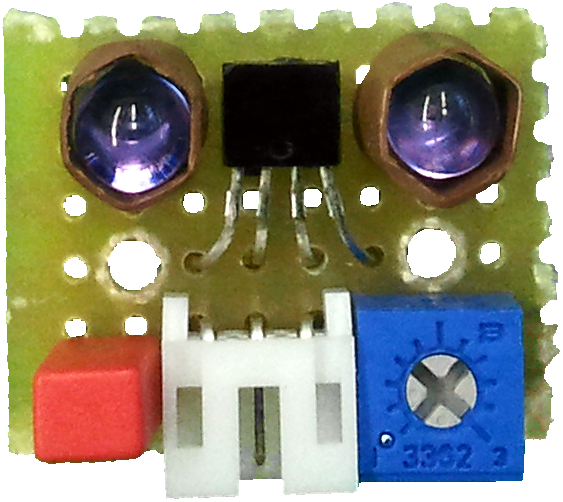
\includegraphics[scale=.19]{content/image/hw_quadratisch}
		\captionof{figure}[Hardwarevariante 1 - Quadratisch]{Variante 1 - Quadratisch}
		\label{pic:hardvarevariante1}
	\end{minipage}
	\begin{minipage}[t]{.49\textwidth}
		\centering
		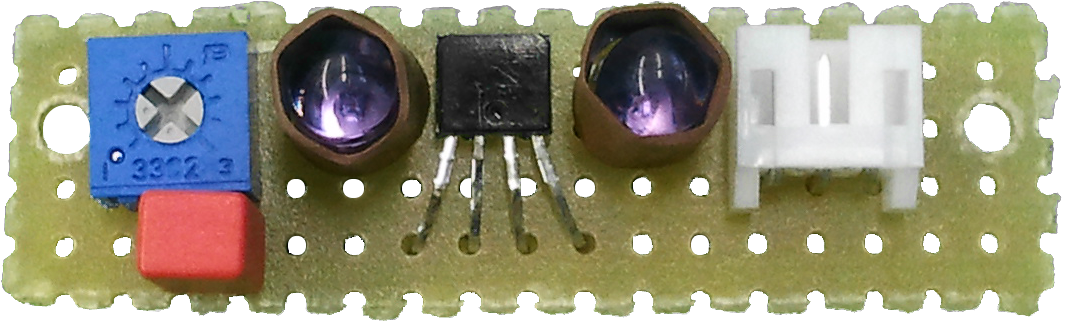
\includegraphics[scale=.19]{content/image/hw_schmal}
		\captionof{figure}[Hardwarevariante 2 - Schmal]{Variante 2 - Schmal}
		\label{pic:hardvarevariante2}
	\end{minipage}
	\end{figure}
	%
	Schlussendlich wurde zusammen die Entscheidung gef�llt beide Varianten zu verwenden. Folgende Konstellation erwies sich als passend:
	
	\begin{description}[leftmargin=!,labelwidth=\widthof{\bfseries Quadratische Version:},noitemsep]
		\item[Schmale Version:] Vorne mittig
		\item[Quadratische Version:] Hinten mittig, vorne rechts und links
	\end{description}
	%
	\section{Software}\label{s:software}
	F�r die Software wird das Echtzeitbetriebssystem FreeRTOS\footnote{Free real-time operating system: \url{http://www.freeRTOS.org/}} verwendet. Beim kleineren Roboter l�uft die Naherkennungs-Software auf dem RoboBoard zusammen mit weiteren Teilgebieten.
	%
		\subsection{Set\_SRF08\_address}\label{ss:set_srf08_address}
		Damit am gleichen \iic-Bus beide Ultraschallsensoren verwendet werden k�nnen, musste zuerst eine separate Software zum �ndern der Slave-Adresse erstellt werden. Der Ablauf der folgende:
		\begin{enumerate}
			\item �berpr�ffen ob neue Adresse g�ltig ist. Falls nicht, Programm nicht fortsetzten.
			\item Erste Pr�fsequenz zur Adress�nderung via \iic\ an Kommandoregister senden und definierte Zeit warten.
			\item Zweite Pr�fsequenz zur Adress�nderung via \iic\ an Kommandoregister senden und definierte Zeit warten.
			\item Dritte Pr�fsequenz zur Adress�nderung via \iic\ an Kommandoregister senden und definierte Zeit warten.
			\item Neue Adresse via \iic\ an Kommandoregister senden.
			\item Beim Aus- und erneuten Einstecken sollte nun die LED auf dem Modul mit dem zur neuen Adresse geh�renden Code (siehe Spezifikationen \cite{url:spec_srf08}) blinken.
		\end{enumerate}
		%
		Der vordere Sensor behielt seine Standard-Adresse (\hex{E0}), dem hinteren wurde die Adresse \hex{E2} neu zugewiesen.
		%
		\subsection{Rangefinder}\label{ss:rangefinder}
		F�r die Naherkennung wurden zwei Task implementiert, einer f�r die Infrarot- und einer f�r die Ultraschallsensoren.
		%
			\subsubsection{IR-Task}\label{sss:ir-task}
			Da ein Infrarotsensor lediglich einen GPIO\footnote{General purpose input/output} ben�tigt, ist der Taskablauf leicht zusammengefasst:
			\begin{enumerate}
				\item GPIOs initialisieren.
				\item Endlosschlaufe des folgenden Ablaufs:
				\begin{enumerate}
					\item Alle vier GPIOs lesen.
					\item �berpr�fen ob einer davon ein Hindernis erkennt.
					\begin{enumerate}
						\item Falls ein Hindernis erkannt ist, IR-Alarmflag setzen.
						\item Andernfalls IR-Alarmflag zur�cksetzen.
					\end{enumerate}
					\item Definierte Zeit warten, so dass der Task immer im gleichen Takt ausgef�hrt wird.
				\end{enumerate}
			\end{enumerate}
			%
			\subsubsection{US-Task}\label{sss:us-task}
			Der Task f�r die Ultraschallsensoren ist etwas komplizierter, wesshalb die Darstellung als Flussdiagram besser geeignet ist. F�r den \iic-Zugriff wurde das Mutex-Verfahren\footnote{Mit dem Mutex-Verfahren kann der gleichzeitige Zugriff mehrerer Tasks auf die selbe Schnittstelle verhindert werden.} verwendet, zur �berschaubarkeit zeit das Diagramm diesen Teil jedoch nicht.
			\image{content/image/flussdiagramm_us-task}{scale=1}[Flussdiagramm des US-Tasks][Flussdiagramm des US-Tasks][pic:flussdiagramm_us-task]
			\clearpage
			%
				\paragraph{Funktion setSRF08Range und setSRF08Gain}\label{par:setsrf08range_setsrf08gain}
				Diese Funktionen dienen dem einmaligen Einstellen der maximalen Reichweite und Verst�rkung. 
				%
				\par F�r die \textbf{Reichweite} wird zuerst der �bergebene Wert auf den zul�ssigen Bereich angepasst. Anschliessend wird der Registerwert mit folgender Formel berechnet und per \iic\ an das Modul geschickt. F�r dieses Projekt wird momentan der Standardwert verwendet.
				\formula{
					x&=\frac{s - \SI{43}{\milli\meter}}{\SI{43}{\milli\meter}}
				}{
					$x$ & Registerwert (\SI{1}{Byte})\\
					$s$ & Reichweite in Millimeter
				}[eq:gain]
				Als maximale Reichweite wird in dieser Version \SI{1}{\meter} verwendet. Im Header-File\footnote{"`src/application/Rangefinder.h"'} ist daf�r ein Makro\footnote{"`RANGEFINDER\_RANGE"'} definiert mit dem der Werte schnell angepasst werden kann.
				%
				\par Der Registerwert der \textbf{Verst�rkung} kann durch Probieren auf die Anwendung angepasst werden. In der Funktion wird wie bei der Reichweite zuerst der Wert �berpr�ft, gegebenenfalls angepasst und dann an das Modul geschickt.
				%
				\paragraph{Funktion startSRF08Meas und readSRF08Meas}\label{par:startsrf08meas_readsrf08meas} Diese Funktionen dienen zur Durchf�hrung einer Messung.
				%
				\par Mit der Funktion \textbf{startSRF08Meas} wird das Kommando zum Starten der Messung in Millimeter per \iic\ an das Modul geschickt. Danach muss eine gewisse Zeit gewartet werden, da das Modul die Echos abwartet und in dieser Zeit nicht verwendet werden kann. F�r das Modul SRF08 mit Standardverst�rkung ist diese Zeit \SI{65}{\milli\second}.\par Nach dem Warten liefert die Funktion \textbf{readSRF08Meas} die gemessene Distanz in Millimeter. Das Modul sendet den Wert in zwei Byte, diese m�ssen also noch zusammengef�gt werden.
				\image{content/image/flussdiagramm_readsrf08meas}{scale = 1, trim = 0 25px 0 25px, clip}[Flussdiagramm der Funktion readSRF08Meas][Flussdiagramm der Funktion readSRF08Meas][pic:flussdiagramm_readsrf08meas]
		%
